\documentclass{article}
\usepackage{amsmath}
\usepackage{pgfplots}
\pgfplotsset{compat=1.16}
\begin{document}
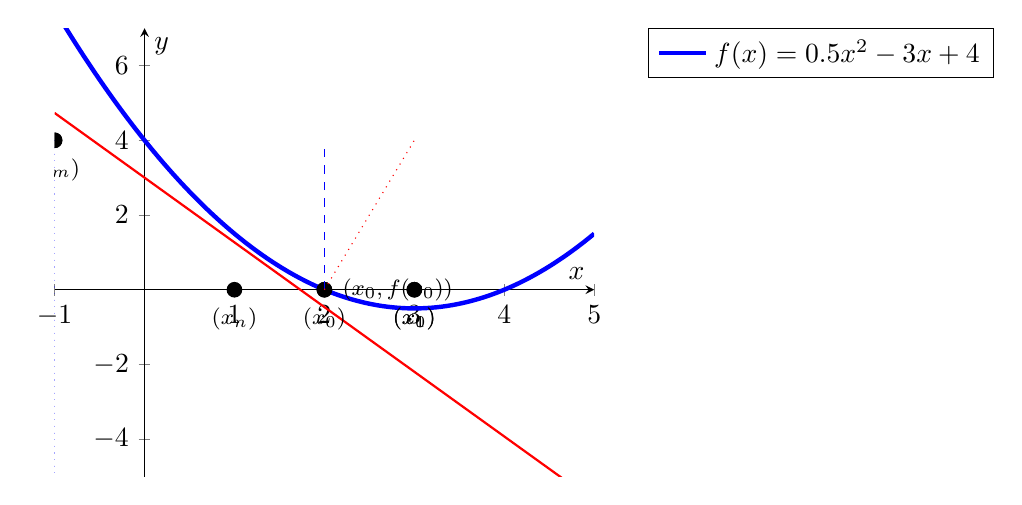
\begin{tikzpicture}
    \begin{axis}[%
        axis lines=center,
        xmin=-1,xmax=5,ymin=-5,ymax=7,
        xlabel={$x$},
        ylabel={$y$},
        legend style={at={(1.1,1)},anchor=north west},
        domain=-1:5
        ]
        \addplot [color=blue,samples=100,ultra thick] {0.5*x^2-3*x+4};
        \addlegendentry{$f(x)=0.5x^{2}-3x+4$}
        \addplot [red,thick,domain=-1:5]{(-3+sqrt(3)*x)/(-1)};
        \draw [blue,dotted] (axis cs:-1,4)--(axis cs:-1,-5);
        \node[circle,fill,inner sep=2pt,label=left:{\footnotesize$(x_{m},f(x_{m}))$}] at(axis cs:-1,4){};
        \node[circle,fill,inner sep=2pt,label=below:{\footnotesize$(x_{m})$}] at(axis cs:-1,4){};
        \node[circle,fill,inner sep=2pt,label=below:{\footnotesize$(x_{n})$}] at(axis cs:1,0){};
        \node[circle,fill,inner sep=2pt,label=right:{\footnotesize$(x_{0},f(x_{0}))$}] at(axis cs:2,0){};
        \node[circle,fill,inner sep=2pt,label=below:{\footnotesize$(x_{0})$}] at(axis cs:2,0){};
        \draw[blue,dashed] (axis cs:2,0)--(axis cs:2,4);
        \draw[densely dashed] (axis cs:2,0)--(axis cs:1,0);
        \draw[red,dotted] (axis cs:2,0)--(axis cs:3,4);
        \node[circle,fill,inner sep=2pt,label=below:{\footnotesize$(x_{1})$}] at(axis cs:3,0){};
        \node[circle,fill,inner sep=2pt,label=below:{\footnotesize$(x_{0})$}] at(axis cs:3,0){};
        \end{axis}
\end{tikzpicture}
\end{document}